
\documentclass[paper=a4,12pt,DIV16,BCOR8mm,twoside]{scrreprt}

\usepackage[utf8]{inputenc}
\usepackage[T1]{fontenc}
\usepackage{lmodern}
\usepackage[english]{babel}

\usepackage[pdftex]{graphicx}
\usepackage{xspace}
\usepackage{textcomp}

% needed for FloatBarrier
\usepackage[section]{placeins}

\usepackage{verbatim}
\usepackage[nomargin,inline,draft]{fixme}

\usepackage{comment}

%\usepackage[firstpage]{draftwatermark}
%\SetWatermarkScale{4}

\usepackage{amsmath}
\usepackage{amssymb}
\usepackage{amsthm}
\usepackage{txfonts}
\usepackage{mathtools}

\usepackage{booktabs}
\usepackage{rotating}
\usepackage{multicol}
\usepackage{multirow}
\usepackage{multicol}


\usepackage{listings}
%Defining C-Code Environment

\usepackage{courier} 
\usepackage{listings}
\usepackage{color} 

% fix bug with listing under texlive-2014
% see https://lists.debian.org/debian-tex-maint/2014/06/msg00209.html

\makeatletter
\renewcommand\lstinline[1][]{%
  \leavevmode\bgroup % \hbox\bgroup --> \bgroup
  \def\lst@boxpos{b}%
  \lsthk@PreSet\lstset{flexiblecolumns,#1}%
  \lsthk@TextStyle
  \ifnum\iffalse{\fi`}=\z@\fi
  \@ifnextchar\bgroup{%
  \ifnum`{=\z@}\fi%
  \afterassignment\lst@InlineG \let\@let@token}{%
  \ifnum`{=\z@}\fi\lstinline@}}
\makeatother

% 1.3.10 jb:
% commented-out unused colors and styles,
% changed color names to logical ones

%\definecolor{darkred}		{rgb}{0.60,0.00,0.00}
\definecolor{coACSLBehavior}	{rgb}{0.30,0.00,0.00}
\definecolor{coASCL}		{rgb}{0.00,0.10,0.00}
\definecolor{coASCLKeyword}	{rgb}{0.00,0.10,0.10}
\definecolor{darkgreen}		{rgb}{0.00,0.40,0.00}
\definecolor{darkblue}		{rgb}{0.00,0.00,0.60}
\definecolor{coCKeyword}	{rgb}{0.00,0.00,0.60}
%\definecolor{red}		{rgb}{0.98,0.00,0.00}
%\definecolor{lightblue}        {rgb}{0.60,0.80,1.00}
%\definecolor{lightred}		{rgb}{1.00,0.60,0.60}

\lstdefinestyle{acsl-block}
{
  emph=[1]{assert, assumes, assigns, axiom, axiomatic, decreases, ensures,
                 ghost, invariant, lemma, logic, loop, predicate,
		 reads, requires, variant},
  emphstyle=[1]{\bfseries\color{coASCLKeyword}},
  emph=[2]{behavior, behaviors, complete, disjoint, for:},
  emphstyle=[2]{\bfseries\color{coACSLBehavior}},
  emph=[3]{typedef, int, char, integer, real, bool, size_type, value_type},
  emphstyle=[3]{\bfseries\color{coCKeyword}},
  escapeinside={//`}{`//},
  morecomment=*[l][\color{coASCL}]{//@},
  morecomment=*[s][\color{coASCL}]{/*@}{*/},
  moredelim=*[is][\bfseries]{|*}{*|}
  %emphstyle=[3]{\ttfamily}
  }

\lstdefinestyle{func-decl}
{
  emph=[1]{assert, assumes, assigns, axiom, axiomatic, decreases, ensures,
                 ghost, invariant, lemma, logic, loop, predicate,
		 reads, requires, variant},
  emphstyle=[1]{\bfseries\color{coASCLKeyword}},
  emph=[2]{behavior, behaviors, complete, disjoint, for:},
  emphstyle=[2]{\bfseries\color{coACSLBehavior}},
  emph=[3]{integer, real, size_type, value_type},
  emphstyle=[3]{\bfseries\color{coCKeyword}},
  escapeinside={//`}{`//},
  morecomment=*[l][\color{coASCL}]{//@},
  morecomment=*[s][\color{coASCL}]{/*@}{*/},
  moredelim=*[is][\bfseries]{|*}{*|},
     frame=none,
     numbers=none
  %emphstyle=[3]{\ttfamily}
}

\lstdefinestyle{acsl-inline}
{
  emph=[1]{assert, assumes, axiom, axiomatic, decreases, ensures,
           ghost, invariant, lemma, logic, loop,
           predicate, reads, requires, return, variant },
  emphstyle=[1]{\bfseries\color{coASCLKeyword}},
  emph=[2]{behavior, behaviors, complete, disjoint, for:},
  emphstyle=[2]{\bfseries\color{coACSLBehavior}},
  emph=[3]{typedef, int, char, integer, real, bool, size_type, value_type},
  emphstyle=[3]{\bfseries\color{coCKeyword}},
  morecomment=*[l][\color{coASCL}]{//@},
  morecomment=*[s][\color{coASCL}]{/*@}{*/},
  moredelim=*[is][\bfseries]{|*}{*|}
}

\lstdefinestyle{inline}
{
  basicstyle = \ttfamily\small\color{coASCL},
  keywordstyle = \ttfamily\small\color{coASCL},
  stringstyle=\color{coASCL},
  style=acsl-inline,
  breaklines= false
}

\lstset
{%
  language=C++,
  defaultdialect=ansi,
  basicstyle=\small\ttfamily,
  commentstyle=\small\color{darkgreen},
  keywordstyle=\small\bfseries\color{darkblue},
  stringstyle=\small\color{darkgreen},
  tabsize = 2,
  showspaces=false,
  showtabs=false,
  columns=fixed,  
  frame=none,  
  breaklines=true,
  showstringspaces=false,
  xleftmargin=0.2cm,
  %rangeprefix=//label, % to specify a certain range from a file
  %rangesuffix=;, % to be shown
  %includerangemarker=false,
  numbers=none
}


\newcommand{\inl}[1]{\lstinline{#1}}

\newcommand{\devicesoft}{\mbox{\textsc{Device-Soft}}\xspace}
\newcommand{\acsl}{\mbox{\textsf{ACSL}}\xspace}
\newcommand{\isoc}{\mbox{\textsf{C}}\xspace}
\newcommand{\macosx}{\mbox{Mac OS X}\xspace}
\newcommand{\framac}{\mbox{\textsf{Frama-C}}\xspace}
\newcommand{\jessie}{\mbox{\textsf{Jessie}}\xspace}
\newcommand{\why}{\mbox{\textsf{Why}}\xspace}
\newcommand{\whythree}{\mbox{\textsf{Why3}}\xspace}
\newcommand{\wpframac}{\mbox{\textsf{WP}}\xspace}
\newcommand{\wpqed}{\mbox{\textsf{Qed}}\xspace}
\newcommand{\altergo}{\mbox{\textsf{Alt-Ergo}}\xspace}
\newcommand{\coq}{\mbox{\textsf{Coq}}\xspace}
\newcommand{\cvc}{\mbox{\textsf{CVC4}}\xspace}

\newcommand{\cealist}{\mbox{\textsf{CEA LIST}}\xspace}
\newcommand{\inria}{\mbox{\textsf{INRIA}}\xspace}
\newcommand{\lri}{\mbox{\textsf{LRI}}\xspace}
\newcommand{\adacore}{\mbox{\textsf{AdaCore}}\xspace}
\newcommand{\sri}{\mbox{\textsf{SRI}}\xspace}
\newcommand{\ansi}{\mbox{\textsf{ANSI/ISO-C}}\xspace}
\newcommand{\xubuntu}{\mbox{\textsf{Xubuntu}}\xspace}

\newcommand{\cxx}{C\nolinebreak[4]\hspace{-.05em}\raisebox{.3ex}{\footnotesize\textbf{++}}\xspace}
% see http://www.parashift.com/c++-faq-lite/misc-environmental-issues.html#faq-40.2

\newcommand{\bitstream}{\texttt{Bitstream}\xspace}
\newcommand{\bitstreamread}{\texttt{Bitstream\_Read}\xspace}
\newcommand{\bitstreamwrite}{\texttt{Bitstream\_Write}\xspace}
\newcommand{\bitstreamnormal}{\inl{NormalBitstream}\xspace}



% to force correct separation of specific words
\hyphenation{non-nega-tive veri-fi-ca-tion simi-lar im-pera-tive com-pari-son col-labo-ra-tion speci-fi-ca-tion fa-mili-ar}

% to give output of the date in the form of month year 
\newcommand{\monthword}[1]{\ifcase#1\or January\or February\or March\or April\or
                                        May\or June\or July\or August\or
                                        September\or October\or November\or December\fi}
\newcommand{\todaymonth}{\monthword{\the\month} \the\year} 


\usepackage{float}
\usepackage{chngcntr}
\counterwithout{footnote}{chapter}

% need to appear as last \usepackage to avoid nonsensical warnings,
% cf. http://mrunix.de/forums/showthread.php?t=38657#8
\usepackage[pdftex]{hyperref}

\floatstyle{plain}
\newfloat{listing}{thp}{lop1}[chapter]
\floatname{listing}{Listing}
\newfloat{predfun}{thp}{lop2}[chapter]
\floatname{predfun}{Listing}


% share counters of all floats:
\makeatletter
\let\c@listing\c@figure
\let\c@predfun\c@figure
%\let\c@lemma\c@figure
\let\c@table\c@figure
\makeatother

% suppress hyperref warnings
\makeatletter
\def\Hy@Warning#1{}
\def\Hy@WarningNoLine#1{}
\makeatother

\renewcommand\floatpagefraction{.95}
\renewcommand\topfraction{.95}
\renewcommand\bottomfraction{.95}
\renewcommand\textfraction{.05}
\setlength{\unitlength}{1mm}

\setlength\topsep{1.5\baselineskip}  % larger space around theorem-like environments

\addtolength{\parskip}{0.5\baselineskip}
\parindent=0cm

\setcounter{tocdepth}{2}
\setcounter{secnumdepth}{2}

\begin{document}

\begin{titlepage}

\begin{center}
\begin{minipage}{0.6\textheight}
\centering
\vspace*{4cm} 
    
\Huge{\textbf{Code Generation and Formal Verification}} \\[1.0cm]
\large{Chapters~7 and~8 of~SUBSET-026} \\[1.2cm]

\Large{\today}\\[1.0cm]

\begin{large}
       Jens Gerlach\\
       Timon Lapawczyk\\[0.5cm]
\end{large}

\vspace*{3cm}
        
%\includegraphics[width=0.40\textwidth]{Figures/FOKUS_4C_CMYK.pdf}

\end{minipage}
\end{center}
\end{titlepage}


%\include{copyright}
%\include{foreword}
%\include{changes}

\listoffixmes
\tableofcontents
\listoffigures
\listof{listing}{List of Code Listings}
%\listof{predfun}{List of Logic Specifications}
%\listoftables

\chapter{Introduction}

\part{Bit Manipulation}



\chapter{The \bitstream Layer}

Conceptually, a \emph{bit stream}~$b$ is a sequence~$b_0,\ldots,b_{n-1}$ of $n$~bits.
Since the \isoc programming language does not allow to directly declare bit sequences
we represent bit streams as \emph{byte arrays}, that is, as arrays of type \inl{uint8_t}
(see Figure~\ref{fig:byte-array}).

\begin{figure}[hbt]
\begin{center}
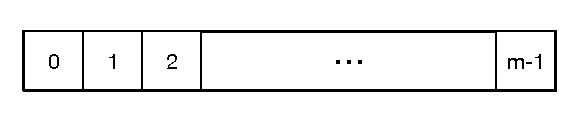
\includegraphics[scale=0.99]{Figures/byte-array.pdf}
\caption{Indexing in a byte array}
\label{fig:byte-array}
\end{center}
\end{figure}

If $x$ is a value of type \inl{uint8_t}, then its uniquely determined binary representation 
\begin{align*}
   x &= \sum_{i = 0}^{7} x_i\cdot 2^i && \text{with } x_k \in \{0, 1\} \text{ for } 0 \leq k < 8
\intertext{suggests an ordering of the bits of $x$ \emph{from the right}, that is, starting with the
position~0 of the \emph{least significant bit} of $x$}
   x &= (x_7,x_6,x_5,x_4,x_3,x_2,x_1,x_0)
\end{align*}

The ETCS standard, however, mandates that numerical values shall be transmitted
starting from the \emph{most significant bit}.
We therefore use the scheme of Figure~\ref{fig:bit-stream} for indexing bits within a byte stream.

\begin{figure}[hbt]
\begin{center}
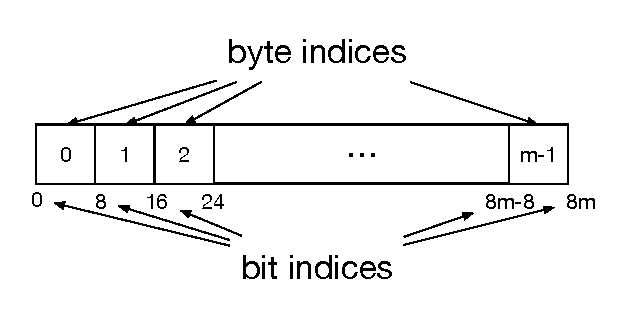
\includegraphics[scale=0.89]{Figures/bit-stream.pdf}
\caption{Indexing in a bit stream}
\label{fig:bit-stream}
\end{center}
\end{figure}

\section{The Type \bitstream and Related Functions}

The type \bitstream in Listing~\ref{lst:bitstream} is our \isoc representation of a bit stream.


\begin{listing}[hbt]
\begin{center}
\begin{lstlisting}[style=acsl-block]
struct Bitstream
{
    uint8_t*  addr;
    uint32_t  size;
    uint32_t  bitpos;
};

typedef struct Bitstream Bitstream;
\end{lstlisting}
\end{center}
\caption{\label{lst:bitstream} Definition of type \bitstream}
\end{listing}

Figure~\ref{fig:bit-stream-type}  shows that for an object of type \bitstream the field \inl{addr} is the
starting address of a byte array of \inl{size} elements and that the field \inl{bitpos}
denotes a bit position within this byte array.

\begin{figure}[hbt]
\begin{center}
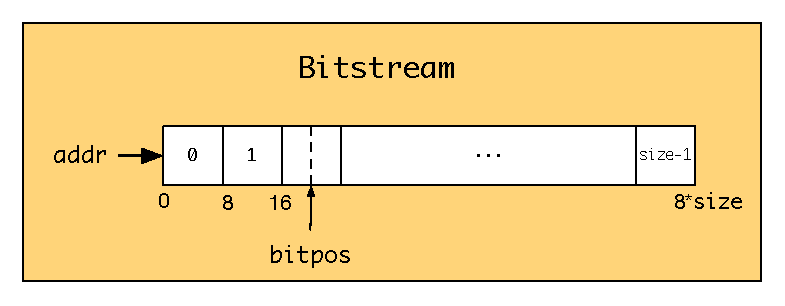
\includegraphics[scale=0.85]{Figures/bit-stream-type.pdf}
\caption{The type \bitstream}
\label{fig:bit-stream-type}
\end{center}
\end{figure}

An obvious type invariant of \bitstream is the condition
\begin{align}
\label{eq:bit-stream-invariant}
    0 \leq \mathtt{bitpos} < 8 \cdot \mathtt{size}
\end{align}

\clearpage

\subsection{The Function \bitstreamread}

The function \bitstreamread, whose declaration is shown in Listing~\ref{lst:bitstream-read-declaration}
reads a sequence of bits from a bit stream and copies the bits into a value of \inl{uint64_t}.


\begin{listing}[hbt]
\begin{lstlisting}[style=acsl-block]
    uint64_t Bitstream_Read(Bitstream* stream, uint32_t length);
\end{lstlisting}
\caption{\label{lst:bitstream-read-declaration} Declaration of \bitstreamread}
\end{listing}

\FloatBarrier

The informal semantics of \bitstreamread is depicted in Figure~\ref{fig:bit-stream-read}.

\begin{figure}[hbt]
\begin{center}
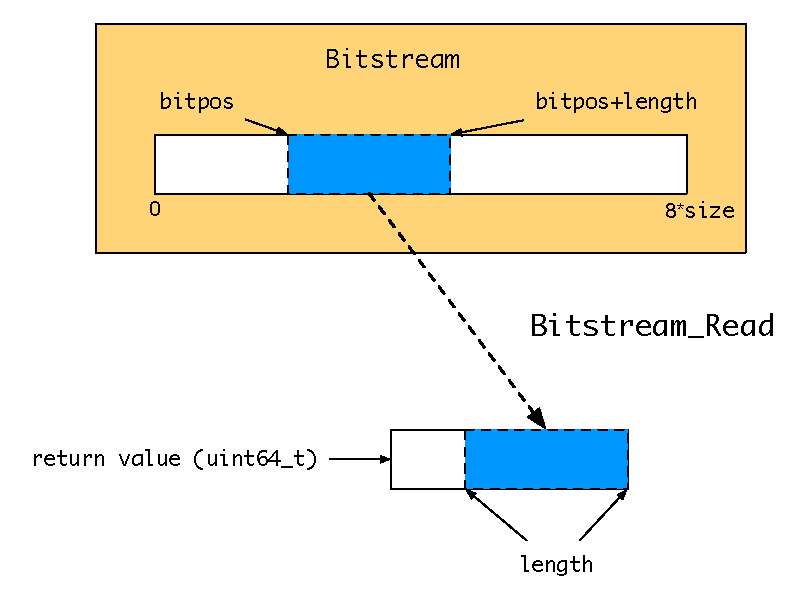
\includegraphics[scale=0.85]{Figures/bit-stream-read.pdf}
\caption{Informal description of \bitstreamread}
\label{fig:bit-stream-read}
\end{center}
\end{figure}

Figure~\ref{fig:bit-stream-read} also suggests the following preconditions of \bitstreamread
\begin{subequations}
\label{eq:bit-stream-read-pre}
\begin{align}
   \mathtt{length} &\leq 64 \\
   \mathtt{bitpos} + \mathtt{length} &\leq 8 \cdot \mathtt{size}
\end{align}
\end{subequations}

\clearpage

\subsection{The Function \bitstreamwrite}

The Function \bitstreamwrite (see Listing~\ref{lst:bitstream-write-declaration})
is, in simple terms, the inverse of \bitstreamread.
It takes \inl{length} bits of the argument \inl{value} and writes it into the bit stream.

\begin{listing}[hbt]
\begin{lstlisting}[style=acsl-block]
    void Bitstream_Write(Bitstream* stream, uint32_t length, 
                         uint64_t value);
\end{lstlisting}
\caption{\label{lst:bitstream-write-declaration} Declaration of \bitstreamwrite}
\end{listing}

The informal semantics of \bitstreamwrite is depicted in Figure~\ref{fig:bit-stream-write}.

\begin{figure}[hbt]
\begin{center}
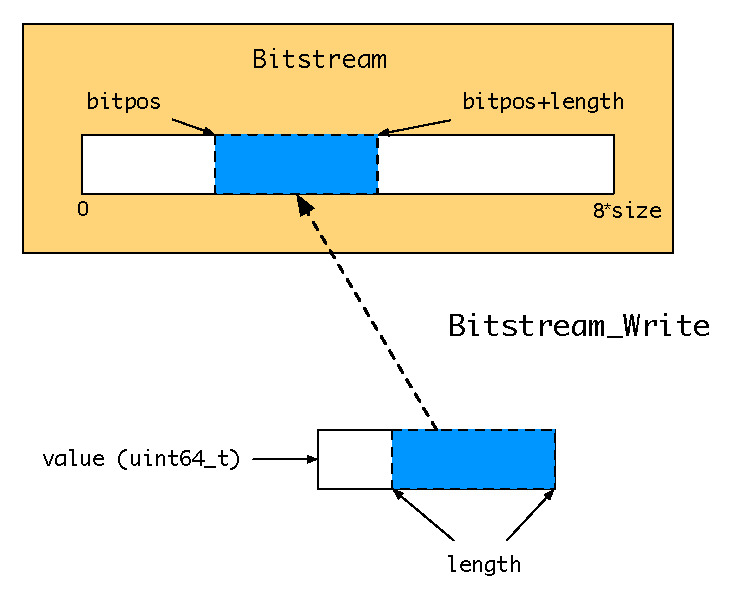
\includegraphics[scale=0.85]{Figures/bit-stream-write.pdf}
\caption{Informal description of \bitstreamwrite}
\label{fig:bit-stream-write}
\end{center}
\end{figure}

In addition to the preconditions~\eqref{eq:bit-stream-read-pre} one must ensure
that the argument \inl{value} can be represented by \inl{length} bits.
In other words, the following precondition must also be satisfied.

\begin{align}
\label{eq:bit-stream-write-pre}
    \mathtt{value} < 2^{\mathtt{length}}
\end{align}

\subsection{The Function \inl{NormalBitstream}}

\section{Predicates}
\subsection{The Predicates \readable and \writeable}
\subsection{The Predicates \invariant and \normal}
\subsection{The Predicates \equalbits and \unchanged}
\subsection{The Predicate \upperbitsnotset}

\section{Formal Specification}
\subsection{The Function \bitstreamread}
\subsection{The Function \inl{Bitstream_Write}}
\subsection{The Function \inl{NormalBitstream}}

\section{Implementation}
\subsection{The Function \bitstreamread}
\subsection{The Function \inl{Bitstream_Write}}
\subsection{The Function \inl{NormalBitstream}}

\section{Formal Verification}
\subsection{\inl{Bitstream_ReadThenWrite}}
\subsection{\inl{Bitstream_WriteThenRead}}



\chapter{The \inl{Bitwalker} Layer}

\section{Predicates}

\section{Formal Specification}
\subsection{The Function \inl{Bitwalker_Peek_Normal}}
\subsection{The Function \inl{Bitwalker_Poke_Normal}}

\section{Implementation}
\subsection{The Function \inl{Bitwalker_Peek_Normal}}
\subsection{The Function \inl{Bitwalker_Poke_Normal}}

\section{Formal Verification}

\chapter{Auxiliary Bit Functions}

\part{Packets from Chapter 7}

\chapter{Packets}

\part{Telegram and Messages from Chapter 8}
\chapter{Eurobalise Telegram}
\chapter{Radio Messages}

\cleardoublepage

%\appendix
%\include{history}
 

% jg:  the "phantomsection" is a hack to fix the wrong reference to bibliography
% see also http://sumanta679.wordpress.com/2009/05/15/latex-list-of-table-list-of-figures-and-bibliography-in-toc/
%\newpage
%\phantomsection \label{listoffig}
%\addcontentsline{toc}{chapter}{Bibliography}
%\bibliographystyle{unsrt}
%\bibliography{bibliography}

\end{document}

